\documentclass{article}
\usepackage[utf8]{inputenc}
\usepackage[T1]{fontenc}
\usepackage{xcolor}
\usepackage{graphicx}

\title{Atividade 02 - Disciplina de Infraestrutura Computacional - Módulo 2}
\author{Luiz Gabriel de Souza}
\begin{document}
\maketitle

\href{https://github.com/Luizgs7/Atividade_pratica_redes_internet_web_DSBD}{Link para o GitHub}


\section{Parte I}

\subsection{Por que “faltam” camadas no roteador e no switch do slide 7?}

Pois o roteador e o switch possuem caracteristicas e objetivos diferentes do ponto de origem e destino.
Além do link e da estrutura física que o switch e o roteador possuem, o destino e a origem precisam de de uma aplicação, que pode ser um device qualquer, como um computador e uma maneira para transportar os dados em uma rede. 
Vale a pena ressaltar que o roteador, diferente do switch, precisa também de um endereço de rede para poder entregar os dados corretamente ao destino.


\subsection{Por que seu roteador Wi-Fi não é um roteador “de verdade”?}
Pois ele não tem a função de rotear as informações que chegam pela rede de fato, quem realiza essa tarefa é o provedor de internet, gerenciando os requests e encontrado as informações necessácias para entregar e receber os dados via rede.


\subsection{Qual a porta padrão dos seguintes protocolos: DHCP, HTTPS e POP3.}
Segue abaixo a porta padrão dos protocolos citados:

\begin{itemize}
    \item \textbf{DHCP:} 67.
    \item \textbf{HTTPS:} 443.
    \item \textbf{POP3:} 110.
\end{itemize}

Fonte: \href{https://pt.wikipedia.org/wiki/Lista_de_portas_dos_protocolos_TCP_e_UDP}


\subsection{Ainda há endereços IPv4 disponíveis no Brasil? Quando esgotaram ou quando esgotarão?}

O estoque disponível de IPv4 para América Latina e Caribe se esgotou em 19/08/2020.
Enquanto isso, os endereços IPv6 estão em constante expansão no Brasil e no mundo. No Brasil, por exemplo, já representa mais de 1/3 do volume total de enderaços. 


Fonte: \href{https://ipv6.br/post/fim-do-ipv4/}


\section{Parte II}

\subsection{Qual o ip local da sua máquina? E da macalan?}
O IPv4 local da minha máquina é o "192.168.41.153" e o IPv6 é o " 2804:214:82e4:ca31:8e1:80d9:7418:9075".

Para a macalan existem 3 diferentes tipos de interfaces de rede, cada qual com seus respectivos IPs:


\begin{itemize}
    \item \textbf{ens19:} Interface de rede associada ao meu usuário, cujo IPv4 é "10.17.110.6" e o IPv6 é o "fe80::216:3eff:fe73:6".
    \item \textbf{eth0:} Interface física de rede que representa a rede Ethernet, usada para conectar com outros computadores numa rede e na internet. Na macalan o IPv4 é o "200.17.202.6" e o IPv6 é o "2801:82:80ff:8001:216:3eff:fe79:6".
    \item \textbf{io:} Interface virtual de rede, geralmente utilizado para diagnósticos e resolução de problemas de rede, e para conectar serviços em servidores locais. Na macalan, o IPv4 é o "127.0.0.1" e o IPv6 é o "::1". 
\end{itemize}


\subsection{Qual a rota padrão da sua máquina? E da macalan?}
A rota de rede padrão da máquina pode ser observado com o comando \textcolor{blue}{route -n} (linux) ou \textcolor{blue}{route PRINT} (windows).

Na minha máquina local a rota padrão ("Default Route") é a "192.168.15.73". Na macalan, existem duas rotas padrão: a "200.17.202.62" e a "200.17.202.3".


\subsection{Qual o caminho (route) mais comum entre sua máquina e a macalan?}

Para encontrar o caminho entre a macalan e a minha máquina, eu usei o comando abaixo dentro da macalan:

\begin{figure}
    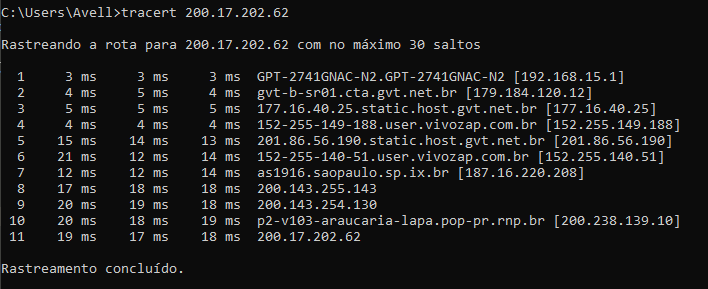
\includegraphics[width=\linewidth]{local_to_macalan_route.PNG}
    \caption{Rota entre minha máquina local a macalan.}
\end{figure}

O resultado indica todo o caminho e o tempo em milisegundos que a minha máquina e a macalan utilizam para se comunicar.
Há referências a endereços da empresa Vivo e GVT que é o meu provedor local, indicando os endereços que os meus dados passam até chegar a macalan.

\subsection{A partir de diferentes máquinas, o caminho (route) até a macalan muda?}

Sim. A rota muda de acordo com o provedor de internet e a localização das máquinas.


\end{document}
